\documentclass[size=a4, parskip=half, titlepage=false, toc=flat, toc=bib, 12pt]{scrartcl}

\setuptoc{toc}{leveldown}

% Ajuste de las líneas y párrafos
\linespread{1.2}
\setlength{\parindent}{0pt}
\setlength{\parskip}{12pt}

% Español
\usepackage[spanish, es-tabla]{babel}

% Matemáticas
\usepackage{amsmath}
\usepackage{amsthm}

% Links
%\usepackage{hyperref}

% Fuentes
\usepackage{newpxtext,newpxmath}
\usepackage[scale=.9]{FiraMono}
\usepackage{FiraSans}
\usepackage[T1]{fontenc}

\defaultfontfeatures{Ligatures=TeX,Numbers=Lining}
\usepackage[activate={true,nocompatibility},final,tracking=true,factor=1100,stretch=10,shrink=10]{microtype}
\SetTracking{encoding={*}, shape=sc}{0}

\usepackage{graphicx}
\usepackage{float}

% Mejores tablas
\usepackage{booktabs}

\usepackage{adjustbox}

% COLORES

\usepackage{xcolor}

\definecolor{verde}{HTML}{007D51}
\definecolor{esmeralda}{HTML}{045D56}
\definecolor{salmon}{HTML}{FF6859}
\definecolor{amarillo}{HTML}{FFAC12}
\definecolor{morado}{HTML}{A932FF}
\definecolor{azul}{HTML}{0082FB}
\definecolor{error}{HTML}{b00020}

% ENTORNOS
\usepackage[skins, listings, theorems]{tcolorbox}

\newtcolorbox{recuerda}{
  enhanced,
%  sharp corners,
  frame hidden,
  colback=black!10,
	lefttitle=0pt,
  coltitle=black,
  fonttitle=\bfseries\sffamily\scshape,
  titlerule=0.8mm,
  titlerule style=black,
  title=\raisebox{-0.6ex}{\small RECUERDA}
}

\newtcolorbox{nota}{
  enhanced,
%  sharp corners,
  frame hidden,
  colback=black!10,
	lefttitle=0pt,
  coltitle=black,
  fonttitle=\bfseries\sffamily\scshape,
  titlerule=0.8mm,
  titlerule style=black,
  title=\raisebox{-0.6ex}{\small NOTA}
}

\newtcolorbox{error}{
  enhanced,
%  sharp corners,
  frame hidden,
  colback=error!10,
	lefttitle=0pt,
  coltitle=error,
  fonttitle=\bfseries\sffamily\scshape,
  titlerule=0.8mm,
  titlerule style=error,
  title=\raisebox{-0.6ex}{\small ERROR}
}

\newtcblisting{shell}{
  enhanced,
  colback=black!10,
  colupper=black,
  frame hidden,
  opacityback=0,
  coltitle=black,
  fonttitle=\bfseries\sffamily\scshape,
  %titlerule=0.8mm,
  %titlerule style=black,
  %title=Consola,
  listing only,
  listing options={
    style=tcblatex,
    language=sh,
    breaklines=true,
    postbreak=\mbox{\textcolor{black}{$\hookrightarrow$}\space},
    emph={jmml@UbuntuServer, jmml@CentOS},
    emphstyle={\bfseries},
  },
}

\newtcbtheorem[number within=section]{teor}{\small TEOREMA}{
  enhanced,
  sharp corners,
  frame hidden,
  colback=white,
  coltitle=black,
  fonttitle=\bfseries\sffamily,
  %separator sign=\raisebox{-0.65ex}{\Large\MI\symbol{58828}},
  description font=\itshape
}{teor}

\newtcbtheorem[number within=section]{prop}{\small PROPOSICIÓN}{
  enhanced,
  sharp corners,
  frame hidden,
  colback=white,
  coltitle=black,
  fonttitle=\bfseries\sffamily,
  %separator sign=\raisebox{-0.65ex}{\Large\MI\symbol{58828}},
  description font=\itshape
}{prop}

\newtcbtheorem[number within=section]{cor}{\small COROLARIO}{
  enhanced,
  sharp corners,
  frame hidden,
  colback=white,
  coltitle=black,
  fonttitle=\bfseries\sffamily,
  %separator sign=\raisebox{-0.65ex}{\Large\MI\symbol{58828}},
  description font=\itshape
}{cor}

\newtcbtheorem[number within=section]{defi}{\small DEFINICIÓN}{
  enhanced,
  sharp corners,
  frame hidden,
  colback=white,
  coltitle=black,
  fonttitle=\bfseries\sffamily,
  %separator sign=\raisebox{-0.65ex}{\Large\MI\symbol{58828}},
  description font=\itshape
}{defi}

\newtcbtheorem{ejer}{\small EJERCICIO}{
  enhanced,
  sharp corners,
  frame hidden,
  left=0mm,
  right=0mm,
  colback=white,
  coltitle=black,
  fonttitle=\bfseries\sffamily,
  %separator sign=\raisebox{-0.65ex}{\Large\MI\symbol{58828}},
  description font=\itshape,
  nameref/.style={},
}{ejer}

% CÓDIGO
\usepackage{listings}

% CABECERAS
\pagestyle{headings}
\setkomafont{pageheadfoot}{\normalfont\normalcolor\sffamily\small}
\setkomafont{pagenumber}{\normalfont\sffamily}

% ALGORITMOS
\usepackage[vlined,linesnumbered]{algorithm2e}
\usepackage{listings}
\usepackage{color}
\renewcommand{\lstlistingname}{Listado}

\definecolor{dkgreen}{rgb}{0,0.6,0}
\definecolor{gray}{rgb}{0.5,0.5,0.5}
\definecolor{mauve}{rgb}{0.58,0,0.82}

\lstset{frame=tb,
  language=Python,
  aboveskip=3mm,
  belowskip=3mm,
  showstringspaces=false,
  columns=flexible,
  basicstyle={\small\ttfamily},
  numbers=none,
  numberstyle=\tiny\color{gray},
  keywordstyle=\color{blue},
  commentstyle=\color{dkgreen},
  stringstyle=\color{mauve},
  breaklines=true,
  breakatwhitespace=true,
  tabsize=2
}

% Formato de los pies de figura
\setkomafont{captionlabel}{\scshape}
\SetAlCapFnt{\normalfont\scshape}
\SetAlgorithmName{Algoritmo}{Algoritmo}{Lista de algoritmos}

% BIBLIOGRAFÍA
%\usepackage[sorting=none]{biblatex}
%\addbibresource{bibliografia.bib}

\begin{document}

\renewcommand{\proofname}{\normalfont\sffamily\bfseries\small DEMOSTRACIÓN}

\title{Trabajo 3\\
Programación}
\subject{Aprendizaje automático}
\author{Johanna Capote Robayna\\
    5 del Doble Grado en Informática y Matemáticas\\
    Grupo A}
\date{}
\publishers{\vspace{2cm}
\includegraphics[height=2.5cm]{UGR}\vspace{1cm}}
\maketitle

\newpage

\tableofcontents
\newpage

\section{Problema de clasificación}

Esta parte de la práctica se desarrolla en el archivo \verb|p3_clasificacion.py|.

\subsection{Problema a resolver}
El problema que se planea consiste en clasificar imágenes de los dígitos del sistema de numeración arábico. Para ello contamos con un dataset (\textit{Optical Recognition of Handwritten Digits Data Set}) en el que se encuentran imágenes ya procesadas de dígitos escritos a mano y nuestro objetivo es predecir dada una nueva imagen de que dígito se trata.

Para procesar las imágenes, en primer lugar cada imagen de 32x32 bits se divide en cuadrados de 4x4 no superpuestos. Cada bit indica si el píxel es blanco o negro. Dentro de cada cuadrado se cuenta el número de píxeles blancos y de píxeles negros, formando así una matriz de 8x8 donde cada elemento es un número entre 0 y 16. Por lo tanto por cada imagen tenemos 64 (8x8) características, donde cada característica es un número entre 0 y 16 que representa el número de píxeles negros o blancos que hay.

Esta base de datos se encuentra distribuida en dos ficheros en formato CSV \verb|optdigits.tra|, donde se encuentra el conjunto de datos de entrenamiento y \verb|optdigits.tes|, donde está el conjunto de \textit{test}. Cada dato consta de 64 características y una etiqueta entre el 0 y 9 que determina el dígito al que corresponden las imágenes. Por lo tanto identificamos los datos del problema como:
\begin{itemize}
\item $X$: $\{0, \dots , 16\}^{64}$
\item $Y$: $\{0, \dots, 9\}$
\item $f$: función que hace corresponder cada vector de características $x \in X$ con su etiqueta correspondiente $y \in Y$.
\end{itemize}

\newpage
\subsection{Selección de las clases de funciones a usar}
Nos encontramos en un problema de clasificación multiclase, por lo que nuestra clase de hipótesis cambia, empleando la ténica \textit{one-versus-all}. Consideramos entonces para cada $i \in \{0,\dots,9\}$ el clasificador binario en el espacio $X$ dado por:
$$h_i(x) = w^{T}x \ , w \in \mathbb{R}^d $$
El cual mide la distancia con signo del punto $x$ al hiperplano definido por $w$, si la distancia es positiva el punto pertenece a la clase $i$ y si es negativa pertenece a cualquiera de las otras clases. Para elegir a que clase pertenece un dato $p(x)$, le asignaremos la clase en la que su distancia sea mayor, es decir:
$$p(x) = \arg \max_i h_i(x) $$
Por lo que la clase de funciones que utilizamos es:
$$H = \left\{ \arg \max_i w_{(i)}^T x : w_{(i)} \in \mathbb{R}^d \ , i = 0, \dots , 9 \right\}$$


\subsection{Conjuntos \textit{training} y \textit{test}}

Como ya comentamos anteriormente, extraemos el conjunto de \texit{training} del archivo \verb|optdigits.tra| y el conjunto \textit{test} del archivo \verb|optdigits.tes|. Como están en formato CSV cada linea se corresponde con un dato y se separan las características por comas. El conjunto de entrenamiento consta de 3823 datos (68.02 \%) mientras que el de test de 1797 (31.98 \%). Consideramos que las particiones son correctas para el problema.

Como nuestro conjunto de entrenamiento no es muy grande, utilizamos la técnica de \textit{cross-validation}, puesto que realizar una segunda división para obtener el conjunto de validación supondría que el conjunto de entrenamiento resultante sea demasiado pequeño. Para ello se utiliza la función \verb|GridSearchCV| de \verb|sklearn| y se divide el conjunto en 5 (\verb|cv=5|), medida recomendada.

\subsection{Preprocesado de datos}
Aunque los datos proporcionados han sido previamente preprocesados comprobamos que no hayan valores perdidos ni fuera de rango. Comprobamos que no haya ningún valor perdido (null) y que todas las características se encuentren en el intervalo $[0,16]$. Además comprobamos que todas las etiquetas se encuentra en el intervalo $[0,9]$.

\begin{verbatim}
Número de valores perdidos en el conjunto de entrenamiento: 0
Número de valores perdidos en el conjunto de test: 0
Valor mínimo de las caraterísticas del conjunto de entrenamiento: 0
Valor máximo de las caraterísticas del conjunto de entrenamiento: 16
Valor mínimo de las caraterísticas del conjunto de test: 0
Valor máximo de las caraterísticas del conjunto de test: 16
Valor mínimo de las etiquetas del conjunto de entrenamiento: 0
Valor máximo de las etiquetas del conjunto de entrenamiento: 9
Valor mínimo de las etiquetas del conjunto de test: 0
Valor máximo de las etiquetas del conjunto de test: 9
\end{verbatim}

Además comprobamos que las clases estén bien balanceadas. En la siguiente imagen podemos ver que las clases tienen entre 350 y 400 muestras cada una y se encuentran bien balanceadas.
\begin{figure}[H]
\centering
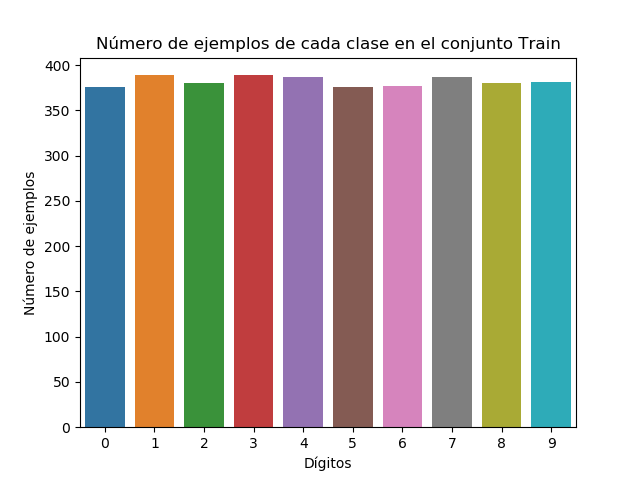
\includegraphics[width=0.7\textwidth]{./img/clasestrain}
\caption{Número de muestras por cada clase en el conjunto de entrenamiento.}
\end{figure}
\begin{figure}[H]
\centering
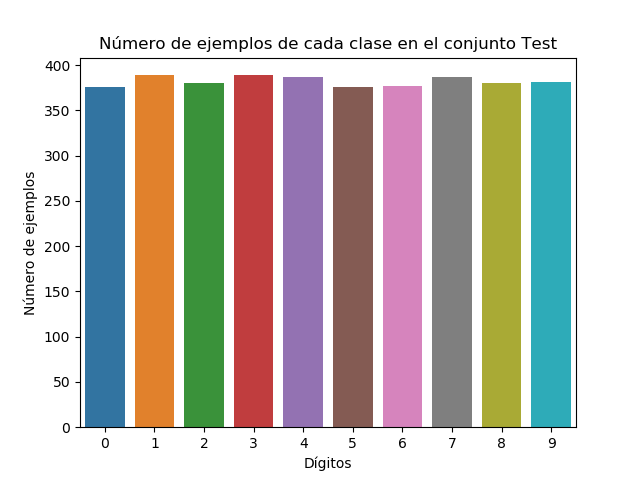
\includegraphics[width=0.7\textwidth]{./img/clasestest}
\caption{Número de muestras por cada clase en el conjunto de test.}
\end{figure}

Para preprocesar los datos utilizamos una estructura \verb|Pipeline| de \verb|sklearn| para agrupar todas las transformaciones. Realizamos dos transformaciones de los datos:
\begin{enumerate}
\item En primer lugar utilizamos la transformación \verb|StandardScaler()| para reescalar los atributos para evitar datos con distintas escalas. Tras estre reescalado los atributos tienen media $0$ y varianza $1$.

\item Además aplicamos el algoritmo PCA, con el conseguimos reducir la dimensionalidad de las características. Se ha fijado que seleccione el número de componentes de modo que la cantidad de varianza que deba explicarse sea mayor del $95\%$, debido a que en nuestro problema puede haber zonas de la imágen que no sean relevantes (esquinas en blanco,...).

\end{enumerate}
Por lo que el Pipeline del preprocesador quedaría de la siguiente forma:
\begin{verbatim}
preprocesado = [("escalado", StandardScaler()),
                ("PCA", PCA(n_components=0.95))]

preprocesador = Pipeline(preprocesado)
\end{verbatim}
Para analizar los logros obtenidos con el preprocesado de datos utilizamos una matriz de correlaciones con la que podemos observar que el preprocesador de datos ha mejorado la correlación de las características. En las siguientes imágenes podemos observar como se ha reduciendo a 41 las características y se han eliminado las correlaciones entre ellas.
\begin{figure}[H]
\centering
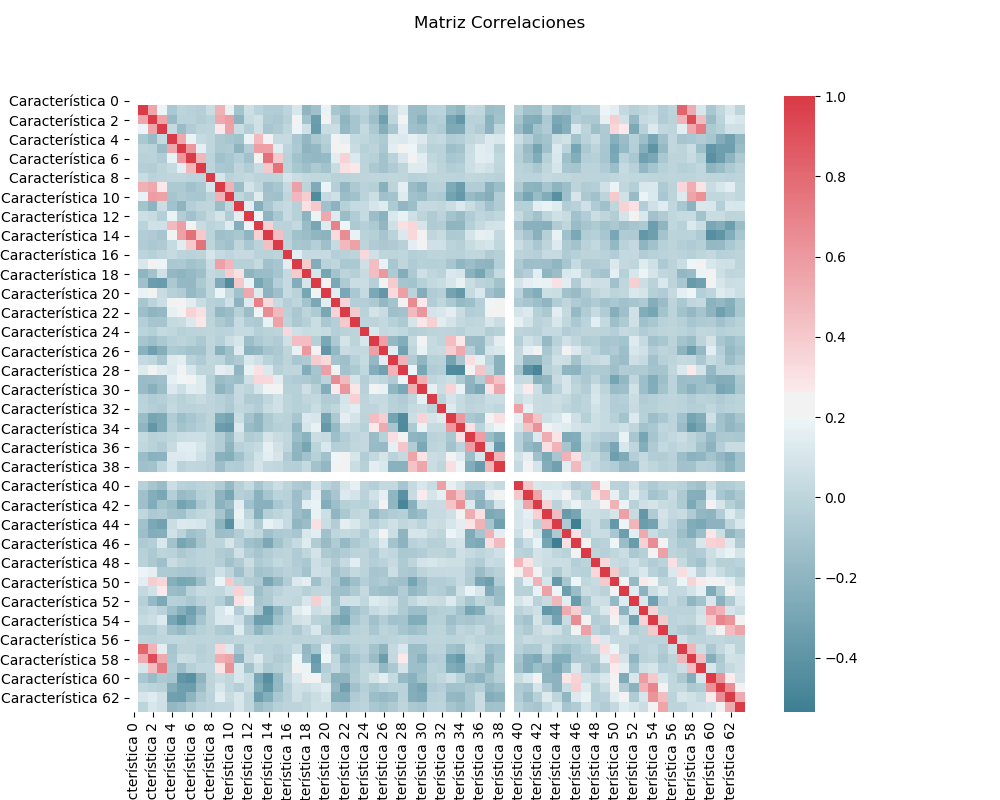
\includegraphics[width=1\textwidth]{./img/antespre}
\caption{Matriz de correlaciones antes del preprocesador de datos.}
\end{figure}
\begin{figure}[H]
\centering
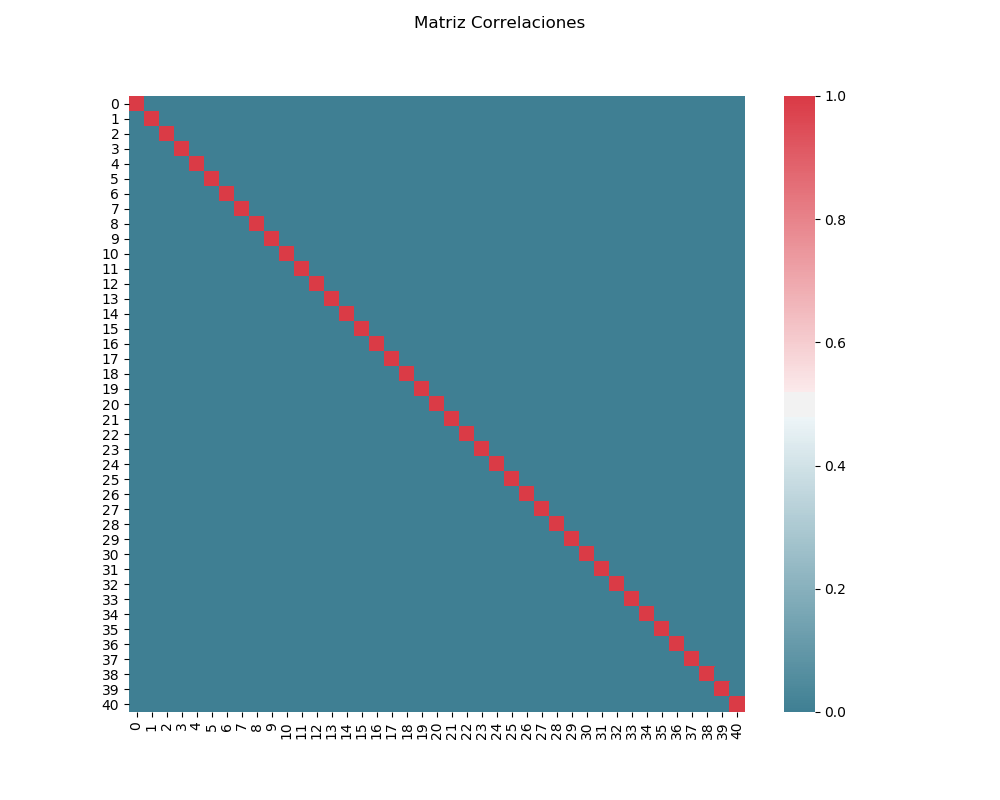
\includegraphics[width=1\textwidth]{./img/despuespre}
\caption{Matriz de correlaciones después del preprocesado de datos.}
\end{figure}

\subsection{Métrica de error}

Como métrica de error utilizaremos el \textit{accuracy}, la usual en este tipo de problemas. Esta medida expresa el error como un valor entre 0 y 1, siendo 0 cuando todos los puntos están bien clasificados y 1 cuando están todos mal clasificados. Para calcularla, dado un $h \in H$ el error viene dado por:
$$E_{in}(h) = \frac{1}{N} \sum_{x_n \in X} [[ h(x) \neq y_n]] $$

Para visualizar y analizar el error utilizamos la matriz de confusión, aunque está no es una medida métrica, la mayoría de métricas se basan en esta matriz. Esta matriz es un método visual en el que podemos ver el rendimiento de un modelo supervisado. Esta matriz muestra los falsos positivos y los verdaderos positivos.

\subsection{Regularización}

Para evitar sobreajustes en el modelo debido a la alta dimensión de nuestro conjunto de datos introducimos técnicas de regularización, las cuales reducen la complejidad de modelo introduciendo un término en la función de coste. Es decir, la regularización reduce la varianza del modelo sin incrementar considerablemente el sesgo de este.

Dentro de todos los métodos de regularización, elegimos la Regularización de Ridge($L_2$) ya que proporciona mejores resultados cuando la mayoría de los atributos son relevantes, como es nuestro caso.

Este método añade una penalización cuadrática en los pesos a la función de pérdida (L):
$$L_{(L_2)}(w) = L(w) + \lambda \|w\|_2^2 $$

\subsection{Ténica de ajuste y módelos}

En primer lugar aclaramos que consideramos como modelos un estimador y un conjunto fijo de hiperparámetros, es decir cada modelos será un estimador y una combinación de sus hiperparámetros.

Los modelos elegidos están expresados en un diccionario, en el cual la parte \verb|'clf'| hace referencia al estimador y \verb|'clf__Parametro|' hace referencia a cada uno de los hiperparámetros del estimador y los valores que toma para cada modelo. Los modelos elegidos son los siguientes:

\begin{itemize}
\spanishdecimal{.}
\item \textbf{Regresión logistica}. Elegimos este modelo porque suele obtener buenos resultados en problemas de clasificación multiclase. Elegimos como ya mencionamos anteriormente la regularización $L_2$, además indicamos que la estratégia de clasificación es la \verb|'ovr'| (\textit{one-vs-rest}) ya explicada en la clases de funciones que buscamos y por último elegimos un número máximo de iteraciones de 1000. Por otro lado hacemos variar el parámetro \verb|C| entre los valores $\{2.0, 1.0, 0.1 , 0.01, 0.001\}$, es decir finalmente habrán cinco modelos formado por cada estimador y su posible valor del parámetro \verb|C|.

\begin{verbatim}
{'clf': [LogisticRegression(penalty='l2', # Regularización Ridge (L2)
               multi_class='ovr', # Indicamos que la regresión logística es multinomial
               solver = 'lbfgs', # Algoritmo a utilizar en el problema de
               # optimización
               max_iter = 1000)],
    'clf__C':[2.0, 1.0, 0.1, 0.01, 0.001]}
\end{verbatim}
En esta caso la técnica de ajuste es la LBFGS, la cual se basa en un método iterativo parecido al método de Newton pero que utiliza una aproximación de la inversa de la matriz Hessiana. La función que optimiza o ajusta este método es la función de pérdida logarítmica a la que se le añade la regularización $L_2$.

\item \textbf{Perceptron}. A este modelo, utilizado ya en la práctica anterior, le establecemos como parámetros la regularización $L_2$, el criterio de parada a $10^{-3}$ e indicamos que las clases están balanceadas.
\begin{verbatim}
{'clf': [Perceptron(penalty = 'l2', # Regularización de Ridge (L2)
                         tol = 1e-3, # Criterio de parada
                         class_weight = "balanced"]},  #clases balanceadas
\end{verbatim}
Como técnica de ajuste este modelo utiliza la técnica iterativa SGD, en el cual se fija un \textit{learning-rate} = 1.
\item \textbf{Ridge}. Este modelo utiliza una regresión lineal añadiéndole la penalización de Ridge ($L_2$). Como parámetros hemos establecido que los datos están normalizados y balanceados y se ha establecido una tolerancia de $0.1$ que es la recomendada. Además hacemos variar el parámetro \verb|alpha| entre los valores $\{1.0, 0.1, 0.01, 0.001 \}$, es decir, finalmente habrá cuatro modelos, cada uno formado por el estimador y cada posible valor del parámetro \verb|alpha|.
\begin{verbatim}
{'clf': [RidgeClassifier(normalize=True, # datos normalizados
                              class_weight="balanced", # clases balanceadas
                              random_state=100,
                              tol=0.1)],
  'clf__alpha': [1.0, 0.1, 0.01, 0.001]}
\end{verbatim}
Como técnica de ajuste este modelo utiliza la técnica de la Pseudoinversa.
\end{itemize}

\subsection{Estimación de hiperparámetros y elección del mejor modelo}

Para seleccionar el mejor modelo utilizamos la función \verb|GridSearchCV| la cual utiliza la técnica de \textit{cross-validation} para entrenar y validar los distintos modelos. Esta función elabora un grid con todas las posibles combinaciones de los diccionarios sin mezclar entre ellos (cada estimador con sus parámetros),por lo que le pasamos el preprocesador y la lista con todos los modelos a probar. A continuación entrenamos el \textit{grid} con la función \verb|fit| y elegimos como nuestro clasificador final el mejor estimador, el cual será el que tenga mejor \textit{accuracy}. Este estimador que nos devuelve el \verb|GridSearchCV| ya está entrenado en todo el conjunto de entrenamiento por lo que no es necesario volverlo a entrenar.
\begin{verbatim}
grid = GridSearchCV(preprocesador, modelos, scoring='accuracy', cv=5,
                    n_jobs = -1)
grid.fit(X, y)
clasificador = grid.best_estimator_
\end{verbatim}

Tras ejecutar esto con nuestra lista de modelos, obtenemos como resultado que el mejor clasificador es la combinación del estimador \verb|LogisticRegression| y el parámetro \verb|C=1.0|.
\subsection{Estimación por validación cruzada del error $E_{out}$}
Una vez elegido el clasificador lo utilizamos en el conjunto de \textit{Test} hallando así el error $E_{test}$. Este error es una estimación de $E_{out}$.
\begin{verbatim}
E_in: 0.029034789432382913
E_test: 0.05898720089037279
\end{verbatim}
Como ya comentamos en la métrica del error, en este problema de clasificación podemos utilizar como método visual para analizar el error la matriz de confusiones en la cual se muestra para cada clase el porcentaje de datos bien clasificados y el porcentaje de etiquetas mal predichas. En la siguiente imagen podemos ver como los porcentajes de aciertos son bastante altos (el más bajo es un 88\% de la etiqueta 8) y que la confusión más grande esta en que la etiqueta 1 la clasifica como un 8.
\begin{figure}[H]
\centering
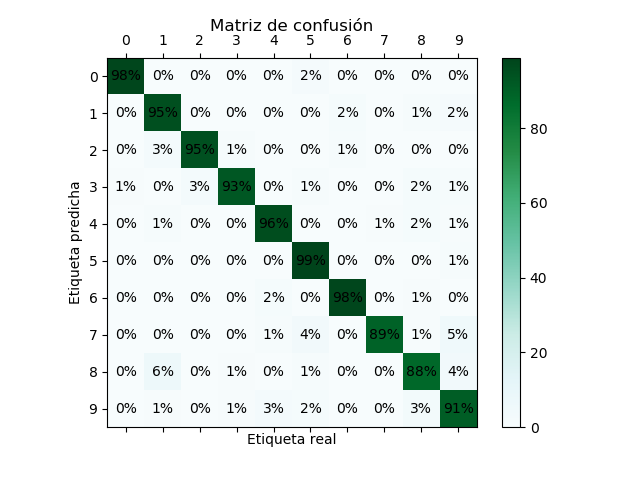
\includegraphics[width=1\textwidth]{./img/confusion}
\caption{Matriz de confusión.}
\end{figure}

Para estimar una cota para el $E_{out}$ utilizamos la cota de \textit{Hoeffding} aplicada sobre el error en nuestro conjunto test, con la cual podemos asegurar con probabilidad $1 - \delta$:
\spanishdecimal{.}
$$E_{out} \leq E_{test} + \sqrt{ \frac{1}{2 N_{test}} \cdot \log \frac{2 M_test}{\delta}} $$
El tamaño del conjunto $N_{test}$ es 1797, por otro lado $M_{test}$ es 1 ya que hemos estimado la solución previamente y hemos elegido una concreta. Por tanto, si fijamos por ejemplo $\delta = 0.05$ tenemos que con una probabilidad del $95\%$:
$$ E_{out} \leq 0.05899 + \sqrt{ \frac{1}{2 \cdot 1797} \cdot \log \frac{2}{0.05}} \approx 0.091$$
Por lo tanto sabemos que con una probabilidad de $95\%$ el $E_{out}$ tomará un valor menor que un $9.1\%$.

\subsection{Modelo propuesto para la empresa}
Si nos ponemos en el contexto de que nos han encargado realizar este ajuste para una empresa, tras todos los procesos mencionados anteriormente elegimos como modelo la \textbf{Regresión logistica} con \textbf{C = 1.0}. Este modelo consigue un buen ajuste el cual hemos podido visualizar en la matriz de confusiones. Se trata de un modelo sencillo y rápido capaz de conseguir un error en el conjunto de \textit{test} del $5.899\%$. Además, por la cota calculada previamente sabemos que el error de generalización no va a superar el $9.1\%$, un error bastante bajo para la mayoría de problemas reales. Probablemente no sea el modelo que proporcione el mejor error, pero de los modelos que se han elegido es el que mejor puntuación ha conseguido.

\newpage
\section{Problema de regresión}

Esta parte de la práctica se desarrolla en el archivo \verb|p3_regresion.py|.

\subsection{Problema a resolver}

El segundo problema que se plantea consiste en predecir el número de crímenes violentos por cada 100000 habitantes en ciertas regiones de EE.UU. Para ello se nos proporciona una base de datos con 128 características, entre las que se recoge información de todo tipo sobre esas regiones como por ejemplo la renta \textit{per cápita}, el porcentaje de familias divorciadas, el número de habitantes, su raza, etc.

De las 128 características cinco son atributos no predictivos (\textit{state}, \texit{county}, \textit{community}, \textit{communityname} y  textit{fold}), los otros 122 son atributos reales entre 0 y 1 y el último (\verb|ViolentCrimesPerPop|) refleja la variable que queremos predecir. Por lo tanto los elementos del problema son los siguientes:
\begin{itemize}
\item $X$: $[0,1]^{122}$
\item $Y$: $[0,1]$
\item $f$: función que asigna a cada ejemplo $x \in X$ la cantidad de crímenes violentos por cada 100000 habitantes $y \in Y$.
\end{itemize}

\subsection{Selección de las clases de funciones a usar}

La clase de funciones a utilizar en este caso son las combinaciones lineales de $X$, como se ha visto en clase.
$$H = \left\{ w_0 + \sum_i w_i x_i : w_i \in \mathbb{R} \right\} $$

\subsection{Conjuntos \textit{training} y \textit{test}}
En este caso solo se nos proporciona un archivo con los datos \verb|communities.data| y otro con los nombres \verb|communiti.names|. El primero de ellos se encuentra en formato CSV, mientras que el segundo consta de varios datos e explicaciones sobre el conjunto de datos, entre ellos los nombres de los atributos.

 En este caso no tenemos particionados los datos, por lo que utilizamos la función \verb|train_test_split()| para el particionamiento.  Elegimos el tamaño del conjunto test del 20\%, medida estándar.

 Al igual que en clasificación, utilizamos \textit{cross-validation} para el conjunto de validación utilizando al igual que antes 5 particiones.
\subsection{Preprocesado de datos}
Para preprocesar los datos, en primer lugar, al igual que en el problema anterior nos fijamos si hay datos perdidos. En este caso si los hay. Decidimos borrar las columnas con algún valor perdido ya que no tenemos la suficiente información como para estimar estos valores.
\begin{verbatim}
Número de valores perdidos en el conjunto de datos: 36851
Número de columnas con valores perdidos: 23
\end{verbatim}

De nuevo, al igual que en el problema de clasificación utilizamos un \verb|Pipeline| para el procesado de datos utilizando las mismas técnicas para reducir la complejidad (PCA) y para escalar los datos (StandardScaler).

\begin{verbatim}
preprocesado = [("escalado", StandardScaler()),
                ("PCA", PCA(n_components=0.95))]

preprocesador = Pipeline(preprocesado)
\end{verbatim}

En las siguiente imágenes podemos ver como antes del preprocesado existía una cantidad considerable de características altamente correlacionadas entre ellas. Además se ha reducido el número de características considerablemente.

\begin{figure}[H]
\centering
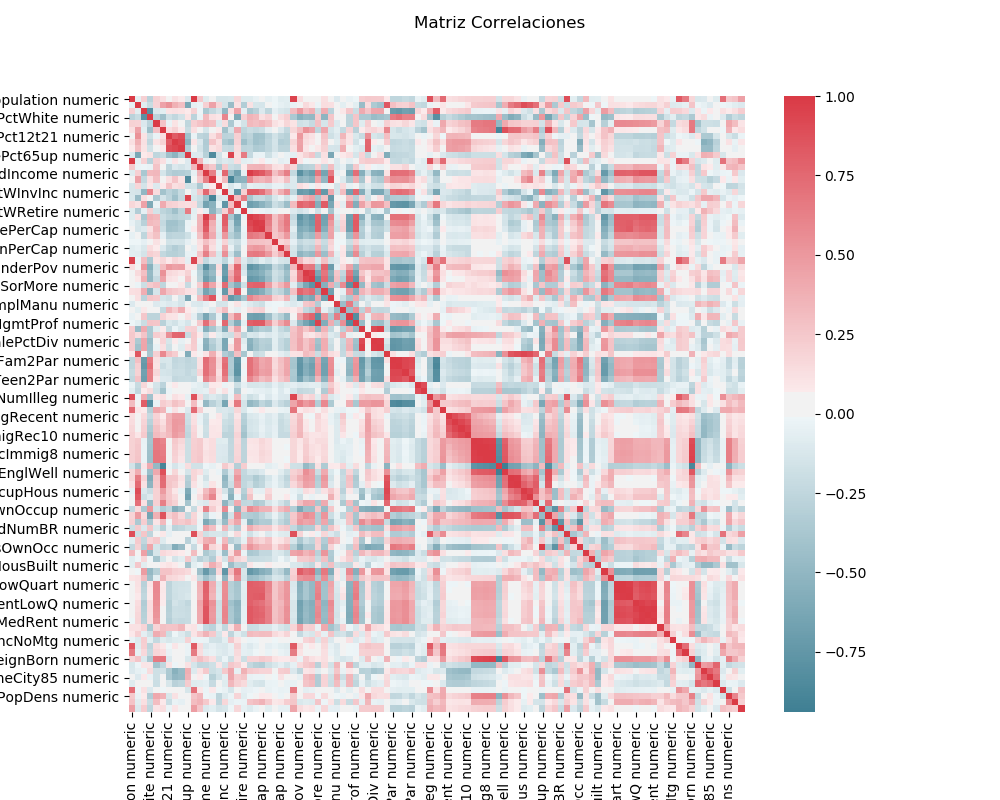
\includegraphics[width=1\textwidth]{./img/corrantereg}
\caption{Matriz de correlaciones antes del preprocesador de datos.}
\end{figure}
\begin{figure}[H]
\centering
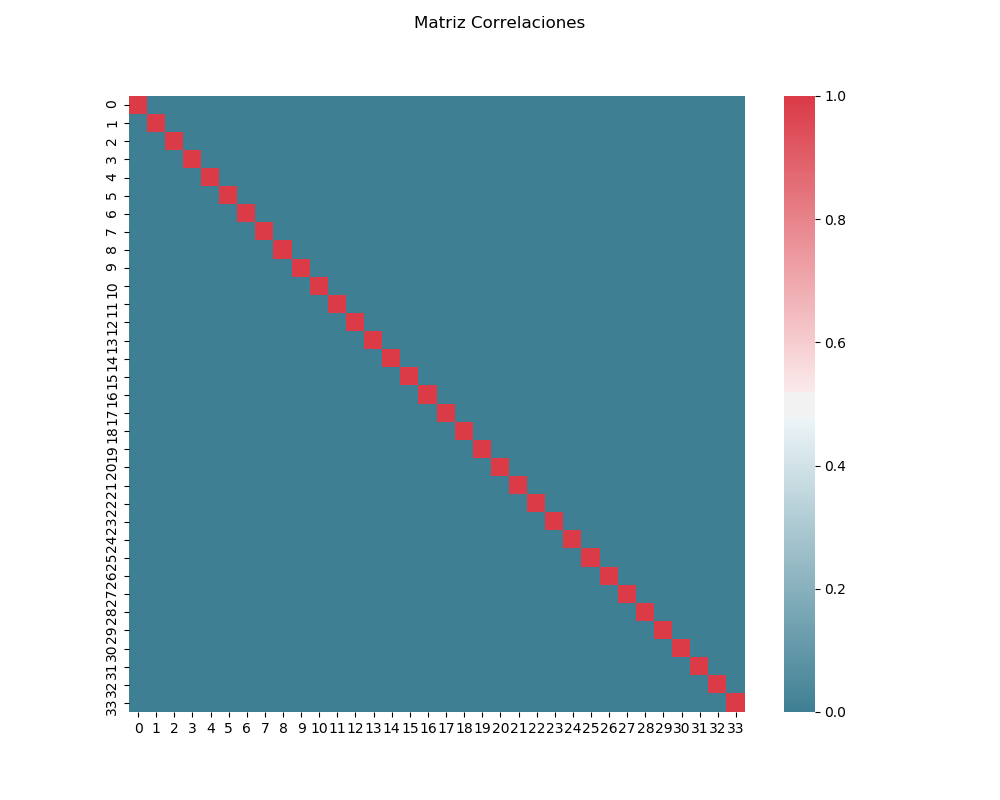
\includegraphics[width=1\textwidth]{./img/corrdespreg}
\caption{Matriz de correlaciones después del preprocesado de datos.}
\end{figure}

\subsection{Métrica de error}

En este caso la métrica que utilizaremos para medir el error es el \texit{coeficiente de determinación} ($R^2$). Está métrica devuelve un valor entre $-\infty$ y 1, siendo $1$ si el modelo predice siempre un valor correcto. Se calcula de la siguiente forma:
$$ R^2 = 1 - \frac{\frac{1}{N} \sum_{i = 1}^N (y_i - \hat{y}_i)}{\frac{1}{N} \sum_{i = 1}^N (y_i - \bar{y})} $$
donde $\hat{y}_i$ es la predicción y $\bar{y}$ es la media de las $y_i$.

\subsection{Regularización}

De nuevo, para evitar el sobreajuste utilizamos métodos de regularización. En este caso aparte del método de Ridge(L2) probamos también el método de Lasso, ya que en este problema al tener mucha caraterísticas puede ser que no hayamos eliminado todas las características no relevantes. Este último añade una penalización lineal a la función de pérdida:
$$L_{(L_1)}(w) = L(w) + \lambda \sum_i |w_i| $$
\subsection{Técnica de ajuste y módelos}

Al igual que en el problema anterior consideramos como modelo un estimador y un conjunto fijo de hiperparámetros. Los modelos elegidos están expresador en un diccionario en el cual la parte \verb|'est'| hace referencia al estimador y \verb|'est_parametro'| hace referencia a cada uno de los hiperparámetros del estimador y los valores que toma para cada modelo. Los modelos elegidos son los siguientes:
\begin{itemize}
\spanishdecimal{.}
\item \textbf{Regresión lineal}. Modelo utilizado en prácticas anteriores.
\begin{verbatim}
{'est': [LinearRegression()]}
\end{verbatim}
Este modelo utiliza como técnica de ajuste la Pseudoinversa.
\item \textbf{SGD}. Este modelo también se ha utilizado en las prácticas anteriores. Como parámetros le hemos fijado un máximo de 1000 iteraciones. Por otro lado variamos el parámetro \verb|alpha| entre los valores $\{1.0, 0.1, 0.01, 0.001, 0.0001 \}$, es decir tenemos finalmente cinco modelos.
\begin{verbatim}
{'est': [SGDRegressor(max_iter=1000, random_state = 100)],
  'est__alpha':[1.0, 0.1, 0.01, 0.001, 0.0001]}
\end{verbatim}
Este modelo utiliza como técnica de ajuste SGD como su propio nombre indica.
\item \textbf{Ridge}. Este modelo ya se utilizo en el problema de clasificación. Se fija a 1000 el número de iteraciones máximas. Y al igual que antes hacemos variar el parámetro \verb|alpha| entre los valores $\{1.0, 0.1, 0.01, 0.001, 0.0001\}$, es decir se construyen cinco modelos.
\begin{verbatim}
{'est': [Ridge(max_iter=1000, random_state = 100)],
  'est__alpha':[1.0, 0.1, 0.01, 0.001, 0.0001]}
\end{verbatim}
\item \textbf{Lasso}. Este modelo utiliza una regresión lineal añadiendole la penalización de Lasso ($L_1$). Se ha establecido un número máximo de iteraciones de 1000. Además variamos el parámetro \verb|alpha| entre los valores $\{1.0, 0.1, 0.01, 0.001, 0.0001\}$, formando cinco modelos.
\begin{verbatim}
{'est': [Lasso(max_iter=1000, random_state = 100)],
'est__alpha':[1.0, 0.1, 0.01, 0.001, 0.0001]}
\end{verbatim}
Este modelo basa su técnica de ajuste en el algoritmo SGD.
\end{itemize}
\subsection{Estimación de hiperparámetros y elección del mejor modelo}

Al igual que en el problema de clasificación, para seleccionar el mejor modelo utilizamos la ténica \textit{cross-validation} llamando a la función \verb|GridSearchCV| el cual elabora un grid con todas las posibles combinaciones de los diccionarios sin mezclar entre ellos (cada estimador con sus parámetros). A esta función le pasamos el preprocesador y la lista de los modelos. A continuación entrenamos el \textit{grid} con la función de \verb|fit| y elegimos como estimador final aquel con mejor puntuación $R^2$. Este estimador que nos devuelve el \verb|GridSearchCV| ya está entrenado en todo el conjunto de entrenamiento por lo que no es necesario volverlo a entrenar.
\begin{verbatim}
grid = GridSearchCV(preprocesador, modelos, scoring='r2', cv=5)
grid.fit(X_train,y_train)
predictor = grid.best_estimator_
\end{verbatim}
Tras ejecutarlo con la lista de modelos comentados anteriormente obtenemos como resultado que el mejor estimador es \verb|Lasso| con el parámetro  \verb|alpha=0.001|.
\subsection{Estimación por validación cruzada del error $E_{out}$}
Una vez obtenido el mejor estimador lo utilizamos como predictor del conjunto \textit{Test}, obteniendo así el error $E_{test}$, con este error aproximamos el valor de $E_{out}$.
\begin{verbatim}
E_test: 0.3336
\end{verbatim}
Para este tipo de problemas no hemos estudiado ninguna cota para el error $E_{out}$, por lo que lo único que podemos decir es que éste será parecido al $E_{test}$.
\subsection{Modelo propuesto para la empresa}
Si nos ponemos en el contexto de que nos han encargado realizar este ajuste para una empresa, tras todos los procesos mencionados anteriormente elegimos como modelo la \textbf{Lasso} con \textbf{alpha = 0.001}. Este estimador obtiene un error de $0.3336$, bajo sabiendo que un regresor que estima simplemente la media de los datos obtiene un error de 1. Además se trata de un modelo rápido y poco complejo, si a estas características le sumamos el bajo error conseguido, este modelo se convierte en el idóneo para este problema dentro de la clase lineal que hemos estudiado. Al igual que en el problema de clasificación no podemos asegurar que proporcione el mejor error, pero si que es el que mejor puntuación ha obtenido de todos los que se han probado.

%printbibliography

\end{document}
